\section{Analog-Digital-Umsetzer}
\subsection{A/D-Umsetzer}
\subsubsection{}

\begin{figure}[H]
\centering
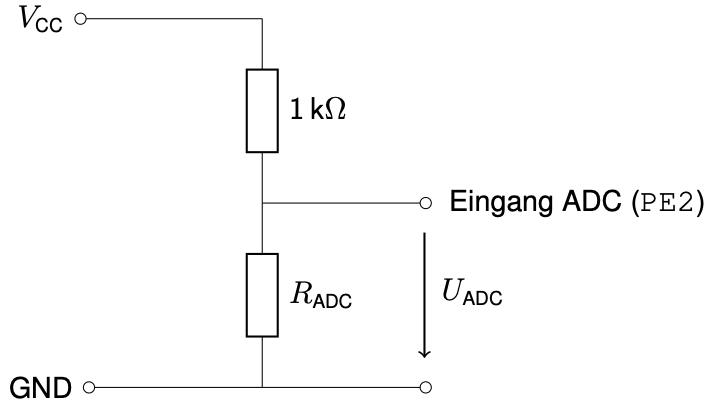
\includegraphics[scale=0.75]{Spannungsteiler.png}
\caption{Schaltbild des Spannungsteilers zur Spannungsmessung}
\label{fig: Spannungsteiler}
\end{figure}

Die Formel zur Berechnung von $U_{\text{ADC}}$ aus \autoref{fig: Spannungsteiler} ist in \autoref{eq: Spannung} gegeben.

\begin{equation}
\label{eq: Spannung}
U_{\text{ADC}}=V_{\text{CC}}\cdot \frac{R_{\text{ADC}}}{1000+R_{\text{ADC}}}
\end{equation}
Die \autoref{tab: Widerstandswerte} zeigt die Widerstandswerte $R_{\text{ADC}}$, sowie die Spannungsabfälle $U_{\text{ADC}}$ über diese Widerstandswerte und die A/D Werte.

\begin{table}[htb]
    \centering
    \caption{Widerstandswerte und dazugehörige Spannungen}
    \label{tab: Widerstandswerte}
    \begin{tabular}{ccc}
        \toprule
        $R_{\text{ADC}}$ [\si{\ohm}]& $U_{\text{ADC}}$  [\si{\volt}] & A/D Wert \\
        \midrule
        \num{100} & \num{0.3} & \num{372} \\
        \num{150} & \num{0.43} & \num{534}\\
        \num{220} & \num{0.60} & \num{738}\\
		\num{680} & \num{1.34} & \num{1658}\\
		\num{1000} & \num{1.65} & \num{2048}\\
		\num{2200} & \num{2.27} & \num{2815}\\
		\num{10000} & \num{3.00} & \num{3724}\\
		\num{15000} & \num{3.09} & \num{3840}\\
        \bottomrule
    \end{tabular}
\end{table}

\subsubsection{}
In \autoref{eq: ADWert} wird der ADC Wert berechnet, wobei $V_{\text{ref}}$  \SI{3.3}{\volt} beträgt.


\begin{equation}
\label{eq: ADWert}
\text{A/D}\; \text{Wert}=\big(2^{12}-1\big)\cdot \frac{U_{\text{ADC}}}{V_{\text{ref}}}
\end{equation}
Die berechneten Werte sind in \autoref{tab: Widerstandswerte} zu finden.

\subsection{Widerstandsmessung}
\autoref{tab: Widerstandsbereiche} zeigt die Widerstandsbereiche und die dazugehörigen A/D-Wertebereiche an.
\begin{table}[htb]
    \centering
    \caption{Widerstandsbereiche und A/D Werte}
    \label{tab: Widerstandsbereiche}
    \begin{tabular}{cccc}
        \toprule
        $R_{\text{ADC,}\,\text{min}}$ [\si{\ohm}]& $R_{\text{ADC}\, \text{max}}$  [\si{\ohm}] & A/D Minimalwert & A/D Maximalwert\\
        \midrule
        \num{0} & \num{100} & \num{0} & \num{372}\\
        \num{101} & \num{150} & \num{373} & \num{534}\\
        \num{151} & \num{220} & \num{535} & \num{738}\\
		\num{221} & \num{680} & \num{739} & \num{1658}\\
		\num{681} & \num{1000} & \num{1659} & \num{2048}\\
		\num{1001} & \num{2200} & \num{2049} & \num{2815}\\
		\num{2201} & \num{10000} & \num{2816} & \num{3723}\\
		\num{10001} & \num{15000} & \num{3724} & \num{3839}\\
        \bottomrule
    \end{tabular}
\end{table}

\begin{lstlisting}
/**
 * main.c
 */
#include<stdint.h>
#include <stdbool.h> // definition of type "bool"
#include"inc/hw_memmap.h" // definition of memory adresses
#include"inc/hw_types.h" // definition of framework makros
#include"driverlib/gpio.h"
#include"driverlib/sysctl.h"
#include<stdint.h>
#include<stdbool.h>
#include"inc/hw_ints.h"
#include"driverlib/timer.h"
#include"driverlib/interrupt.h"
#include "driverlib/debug.h"
#include "driverlib/sysctl.h"
#include "driverlib/adc.h"


//speichert ms seit dem Start
uint32_t systemTime_ms;

void InterruptHandlerTimer0A (void)
{
// Loeschen den Timer-Interrupt, um zu verhindern, dass die Interrupt-Funktion beim Beenden sofort erneut aufgerufen wird
TimerIntClear(TIMER0_BASE, TIMER_TIMA_TIMEOUT);
// eine ms hoch zaehlen
    systemTime_ms++;
}

void clockSetup(void)
{
uint32_t timerPeriod;
//Konfiguriert clock
SysCtlClockSet(SYSCTL_SYSDIV_5|SYSCTL_USE_PLL|SYSCTL_XTAL_16MHZ|SYSCTL_OSC_MAIN);
//Aktiviert peripheral fuer timer
SysCtlPeripheralEnable(SYSCTL_PERIPH_TIMER0);
//konfiguriert timer als 32 bit timer in periodisch mode
TimerConfigure(TIMER0_BASE, TIMER_CFG_PERIODIC);
//setze Zeitperiode auf Anzahl der Perioden, die zum Erzeugen eines
//Timeouts mit einer Frequenz von 1 kHz (alle 1 ms) benoetigt werden
timerPeriod = (SysCtlClockGet()/1000);
// setze TIMER-0-A ein, um nach timePeriod-1-Zyklen ein Timeout zu generieren
TimerLoadSet(TIMER0_BASE, TIMER_A, timerPeriod-1);
//Registriert die Funktion InterruptHandlerTimer0A, die aufgerufen werden soll,
//wenn ein Interrupt von TIMER-0-A auftritt
TimerIntRegister(TIMER0_BASE, TIMER_A, &(InterruptHandlerTimer0A)) ;
//Aktiviert the interrupt fuer TIMER-0-A
IntEnable(INT_TIMER0A);
//erzeugt einen Interrupt , wenn TIMER-0-A ein Timeout sendet
TimerIntEnable(TIMER0_BASE, TIMER_TIMA_TIMEOUT);
//master interrupt aktiviert fuer alle interrupts
IntMasterEnable();
//Aktiviert den Timer, um mit dem Zaehlen zu beginnen
TimerEnable(TIMER0_BASE, TIMER_A);

}

// Es erhaelt als Eingabeparameter die Verzoegerung in ms  und eine Verzoegerung um genau diese Zeit bewirkt.

void delay_ms(uint32_t waitTime) {
//Variable systemTime_ms zaehlt eine Millisekunde hoch und durch die while schleife vergleichen wir der Eingabe Parameter waitTime mit systemTime_ms
// Durch Eingabe der Zahl 500 zaehlt diese funktion bis zu 500 ms und wird jedoch um diese Zeit verzoegert.
    systemTime_ms=0;
    while( systemTime_ms < waitTime);
}
    void delay(void)
    {
      uint32_t i=80000;
      while(i) {i--;}
     }

int main(void){

    SysCtlPeripheralEnable(SYSCTL_PERIPH_GPIOB);                //Set Up
    SysCtlPeripheralEnable(SYSCTL_PERIPH_ADC0);                 // Peripherie aktivieren
    SysCtlPeripheralEnable(SYSCTL_PERIPH_GPIOE);

    GPIOPinTypeADC(GPIO_PORTE_BASE,GPIO_PIN_2);                 // PIN PE2 ADC Funktion zuweisen

    ADCSequenceConfigure(ADC0_BASE,1,ADC_TRIGGER_PROCESSOR,0);  // Prozessor als Trigger Quelle
    ADCSequenceStepConfigure(ADC0_BASE,1,0,ADC_CTL_CH1|ADC_CTL_IE|ADC_CTL_END); // AI1 abtasten/Interrupt erzeugen bei Ende/letzter Schritt
    ADCSequenceEnable(ADC0_BASE,1);                             // ADC Sequenz 1 aktivieren

    GPIOPinTypeGPIOOutput(GPIO_PORTB_BASE, GPIO_PIN_0);         // GPIO Port B Pin 0-7 aktivieren
    GPIOPinTypeGPIOOutput(GPIO_PORTB_BASE, GPIO_PIN_1);
    GPIOPinTypeGPIOOutput(GPIO_PORTB_BASE, GPIO_PIN_2);
    GPIOPinTypeGPIOOutput(GPIO_PORTB_BASE, GPIO_PIN_3);
    GPIOPinTypeGPIOOutput(GPIO_PORTB_BASE, GPIO_PIN_4);
    GPIOPinTypeGPIOOutput(GPIO_PORTB_BASE, GPIO_PIN_5);
    GPIOPinTypeGPIOOutput(GPIO_PORTB_BASE, GPIO_PIN_6);
    GPIOPinTypeGPIOOutput(GPIO_PORTB_BASE, GPIO_PIN_7);
    GPIOPinTypeGPIOInput(GPIO_PORTE_BASE, GPIO_PIN_4);

    bool state = 0;
    uint32_t ui32ADC0Value;

    int R0 = 372;                   //ADC Schwellenwerte
    int R1 = 534;
    int R2 = 739;
    int R3 = 1658;
    int R4 = 2048;
    int R5 = 2816;
    int R6 = 3724;
    int R7 = 3840;

   while(1)
   {

       ADCIntClear(ADC0_BASE,1);                                    // evtl vorhandene ADC Interrupts loeschen
       ADCProcessorTrigger(ADC0_BASE,1);                            // Konvertierung beginnen

       while(!ADCIntStatus(ADC0_BASE,1,false))                      // warten bis Konvertierung abgeschlossen
           {
           }
       ADCSequenceDataGet(ADC0_BASE,1,&ui32ADC0Value);

       if((R1>ui32ADC0Value)&&(ui32ADC0Value>=R0))
       {
           GPIOPinWrite(GPIO_PORTB_BASE, GPIO_PIN_0, GPIO_PIN_0*0xFF);
           delay();
           GPIOPinWrite(GPIO_PORTB_BASE, GPIO_PIN_0, GPIO_PIN_0*0x00);
           delay();
       }

       else if((R2>ui32ADC0Value)&&(ui32ADC0Value>=R1))
           {
           GPIOPinWrite(GPIO_PORTB_BASE, GPIO_PIN_1, GPIO_PIN_1*0xFF);
           delay();
           GPIOPinWrite(GPIO_PORTB_BASE, GPIO_PIN_1, GPIO_PIN_1*0x00);
           delay();
           }

       else if((R3>ui32ADC0Value)&&(ui32ADC0Value>=R2))
           {
           GPIOPinWrite(GPIO_PORTB_BASE, GPIO_PIN_2, GPIO_PIN_2*0xFF);
           delay();
           GPIOPinWrite(GPIO_PORTB_BASE, GPIO_PIN_2, GPIO_PIN_2*0x00);
           delay();
           }
       else if((R4>ui32ADC0Value)&&(ui32ADC0Value>=R3))
           {
           GPIOPinWrite(GPIO_PORTB_BASE, GPIO_PIN_3, GPIO_PIN_3*0xFF);
           delay();
           GPIOPinWrite(GPIO_PORTB_BASE, GPIO_PIN_3, GPIO_PIN_3*0x00);
           delay();
           }
       else if((R5>ui32ADC0Value)&&(ui32ADC0Value>=R4))
           {
           GPIOPinWrite(GPIO_PORTB_BASE, GPIO_PIN_4, GPIO_PIN_4*0xFF);
           delay();
           GPIOPinWrite(GPIO_PORTB_BASE, GPIO_PIN_4, GPIO_PIN_4*0x00);
           delay();
           }
       else if((R6>ui32ADC0Value)&&(ui32ADC0Value>=R5))
           {
           GPIOPinWrite(GPIO_PORTB_BASE, GPIO_PIN_5, GPIO_PIN_5*0xFF);
           delay();
           GPIOPinWrite(GPIO_PORTB_BASE, GPIO_PIN_5, GPIO_PIN_5*0x00);
           delay();
           }

       else if((R7>ui32ADC0Value)&&(ui32ADC0Value>=R6))
          {
           GPIOPinWrite(GPIO_PORTB_BASE, GPIO_PIN_6, GPIO_PIN_6*0xFF);
           delay();
           GPIOPinWrite(GPIO_PORTB_BASE, GPIO_PIN_6, GPIO_PIN_6*0x00);
           delay();
          }
       else if(ui32ADC0Value>R7)
       {
           GPIOPinWrite(GPIO_PORTB_BASE, GPIO_PIN_7, GPIO_PIN_7*0xFF);
           delay();
           GPIOPinWrite(GPIO_PORTB_BASE, GPIO_PIN_7, GPIO_PIN_7*0x00);
           delay();
       }
   }
}
\end{lstlisting}
